\begin{figure}[h]
    \centering
    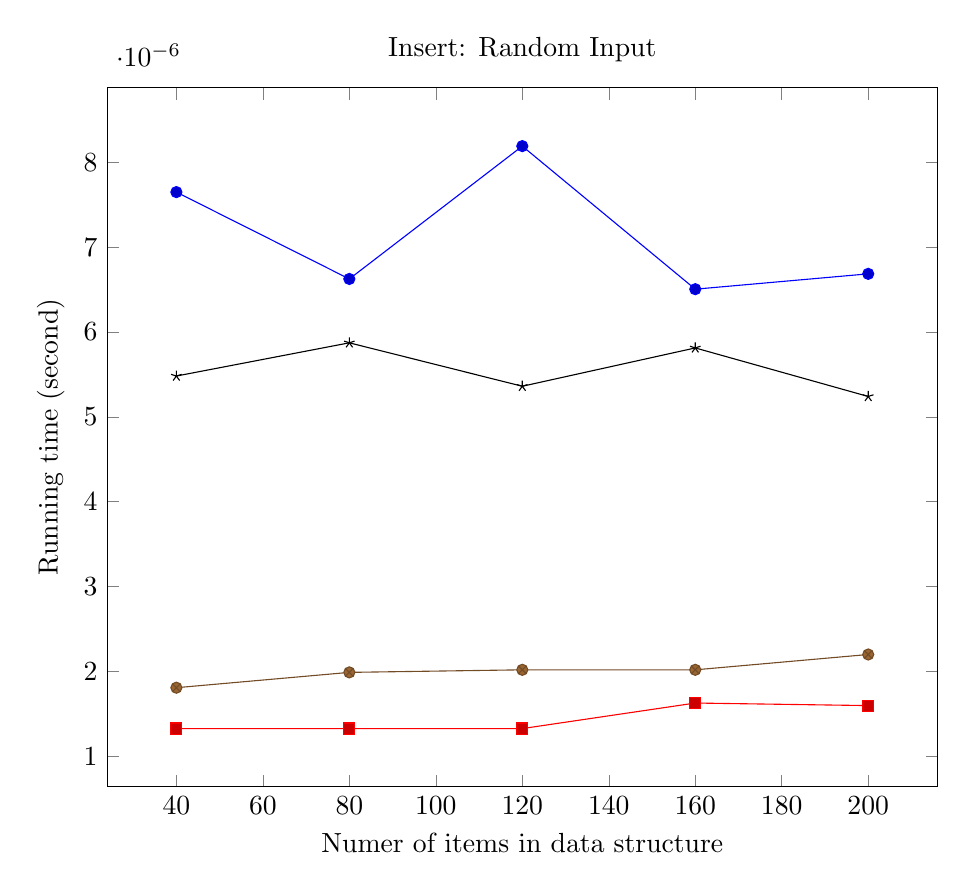
\begin{tikzpicture}
        \begin{axis}[
            xlabel={Numer of items in data structure},
            ylabel={Running time (second)},
            title={Insert: Random Input},
            width=\textwidth
        ]
		\addplot coordinates {
			(40, 7.649853553493013e-06)
			(80, 6.625857408537605e-06)
			(120, 8.191969159643265e-06)
			(160, 6.505387273836316e-06)
			(200, 6.686092475882699e-06)
		};
		\addplot coordinates {
			(40, 1.3251714817086314e-06)
			(80, 1.3251714817086314e-06)
			(120, 1.3251714817086314e-06)
			(160, 1.6263468184618547e-06)
			(200, 1.5962292847837566e-06)
		};
		\addplot coordinates {
			(40, 1.8070520205082374e-06)
			(80, 1.9877572225601716e-06)
			(120, 2.017874756238269e-06)
			(160, 2.017874756238269e-06)
			(200, 2.198579958290203e-06)
		};
		\addplot coordinates {
			(40, 5.481391128880908e-06)
			(80, 5.872919066657323e-06)
			(120, 5.360920994179619e-06)
			(160, 5.812683999306678e-06)
			(200, 5.2404508594783294e-06)
		};
        \legend{}
        \end{axis}
    \end{tikzpicture}
    \caption{Average of 0 operations, benchmarked every 0, starting at 0.}
\end{figure}